
Selected events are required to include exactly three reconstructed light leptons passing the requirement described in \ref{subsec:leps}, which have a total charge of $\pm$1. As the opposite sign lepton is found to be prompt the vast majority of the time \cite{ttH_paper}, it is required to be loose and isolated, as defined though the standard \verb|isolationFixedCutLoose| working point supported by combined performance groups. The same sign leptons are required to be very tight, as per the recommended \verb|isolationFixedCutTight|.

The leptons are ordered in the analysis code as 0, 1, and 2. Lepton 0 is the lepton whose charge is opposite the other two. Lepton 1 is the lepton closest to the opposite charge lepton, i.e. the smallest $\Delta R$, leaving lepton 2 as the lepton further from the opposite charge lepton. Lepton 0 is required to have $p_T > 10$ GeV, while the same sign leptons, 1 and 2, are required to have $p_T > 20$ GeV to reduce the contribution of non-prompt leptons.  

The invariant mass of at least one pair of opposite sign, same flavor leptons is required to fall within 10 GeV of the mass of the Z boson, 91.2 GeV. Events where one of the opposite sign pairs have an invariant mass less than 12 GeV are rejected in order to suppress low mass resonances. %Further, events where the trilepton mass falls within 5 GeV of the Z mass are rejected to remove Z events that include conversions.

An additional requirement is placed on the missing transverse energy, $E^{miss}_T$ > 20 GeV, and the transverse mass of the $W$ candidate, $m(E^{miss}_T + l_{other}) > 30$ GeV, where $E^{miss}_T$ is the missing transverse energy, and $l_{other}$ is the lepton not included in the Z-candidate. 

Events are required to have one or two reconstructed jets passing the selection described in section \ref{subsec:jets}. Events with more than two jets are rejected in order to reduce the contribution of backgrounds such as $t\bar{t}Z$ and $t\bar{t}W$, which tend to have higher jet multiplicity. This selection of summarized in table \ref{tbl:selection}.

\begin{table}[h]
    \centering
    \begin{tabular}{l}
        \hline\hline
        Event Selection\\
        \hline 
        Exactly three leptons with charge $\pm$1 \\
        Two same-charge leptons with $p_T$ $>$ 20 GeV \\
        One opposite charge lepton with $p_T$ $>$ 10 GeV \\
        $m(l^+l^-)$ within 10 GeV of 91.2 GeV \\
        Transverse mass of W-candidate, $m_T(E_T^{miss} + lep_{other})$ $>$ 30 GeV \\
        Missing transverse energy, $E_T^{miss} >$ 20 GeV \\
        One or two jets with $p_T$ $>$ 25 GeV \\
        \hline\hline
    \end{tabular}
    \caption{Summary of the selection applied to events for inclusion in the fit}
    \label{tbl:selection}
\end{table}

%---------------------------
\subsection{Signal Region Validation}
\label{sec:SRkinematics}
%---------------------------

The event yields for both data and Monte Carlo are summarized in table \ref{tab:evt_yields}, which shows good agreement between data and Monte Carlo, and demonstrates that this signal region consists primarily of WZ events.

\begin{table}[H]
    \centering
        \begin{center}
\begin{tabular}{|c|c|}
\hline
Process & Events \\
\hline 
  $WZ + b$   & 167.6 $\pm$ 6.5 \\
  $WZ + c$   & 1080 $\pm$ 40 \\
  $WZ + l$   & 7220 $\pm$ 310 \\
  Other VV   & 850 $\pm$ 140 \\
  $t\bar{t}W$   & 16.8 $\pm$ 2.3 \\
  $t\bar{t}Z$   & 115 $\pm$ 17 \\
  rare Top   & 2.2 $\pm$ 0.1 \\
  Single top   & 0.10 $\pm$ 0.45 \\
  Three top   & 0.01 $\pm$ 0.01 \\
  Four top   & 0.02 $\pm$ 0.01 \\
  $t\bar{t}WW$   & 0.23 $\pm$ 0.05 \\
  $Z+\text{jets}$   & 600 $\pm$ 260 \\
  $V+\gamma$   & 37 $\pm$ 54 \\
  $tZ$   & 190 $\pm$ 70 \\
  $tW$   & 5.5 $\pm$ 1.2 \\
  $WtZ$   & 25.8 $\pm$ 1.1 \\
  $VVV$   & 26.2 $\pm$ 0.9 \\
  $VH$   & 94 $\pm$ 7 \\
  $t\bar{t}$   & 108.68 $\pm$ 8 \\
  $t\bar{t}H$   & 4.3 $\pm$ 0.5 \\
\hline
  Total  & 10600 $\pm$ 530 \\
\hline
  Data   & 10574 \\
\hline 
\end{tabular} 
\caption{Event yields in the preselection region at 139.0 $fb^{-1}$} 
\end{center} 


    %\caption{Data and MC yields after the event selection requiring three leptons, one or two jets, $E^{miss}_T$ > 20 GeV, and $m(E^{miss}_T + l_{other}) > 30$ GeV selection has been applied.}
    \label{tab:evt_yields}
\end{table}

Here Other $VV$ represents diboson processes other than WZ, and consists predominantly of $ZZ\rightarrow llll$ events where one of the leptons is not reconstructed.

Simulations are further validated by comparing the kinematic distributions of the Monte Carlo with data, which are shown in figure \ref{sr_kinematics}.

%textbf{There is some discrepancies between data and MC, particularly in the low MET and low lepton $p_T$ regions, which are being investigated. This is suspected to be the result of underestimating the fake contribution, possibly because of several missing Z+jets simulation files.}

\begin{figure}[H]
    \subfigure[]{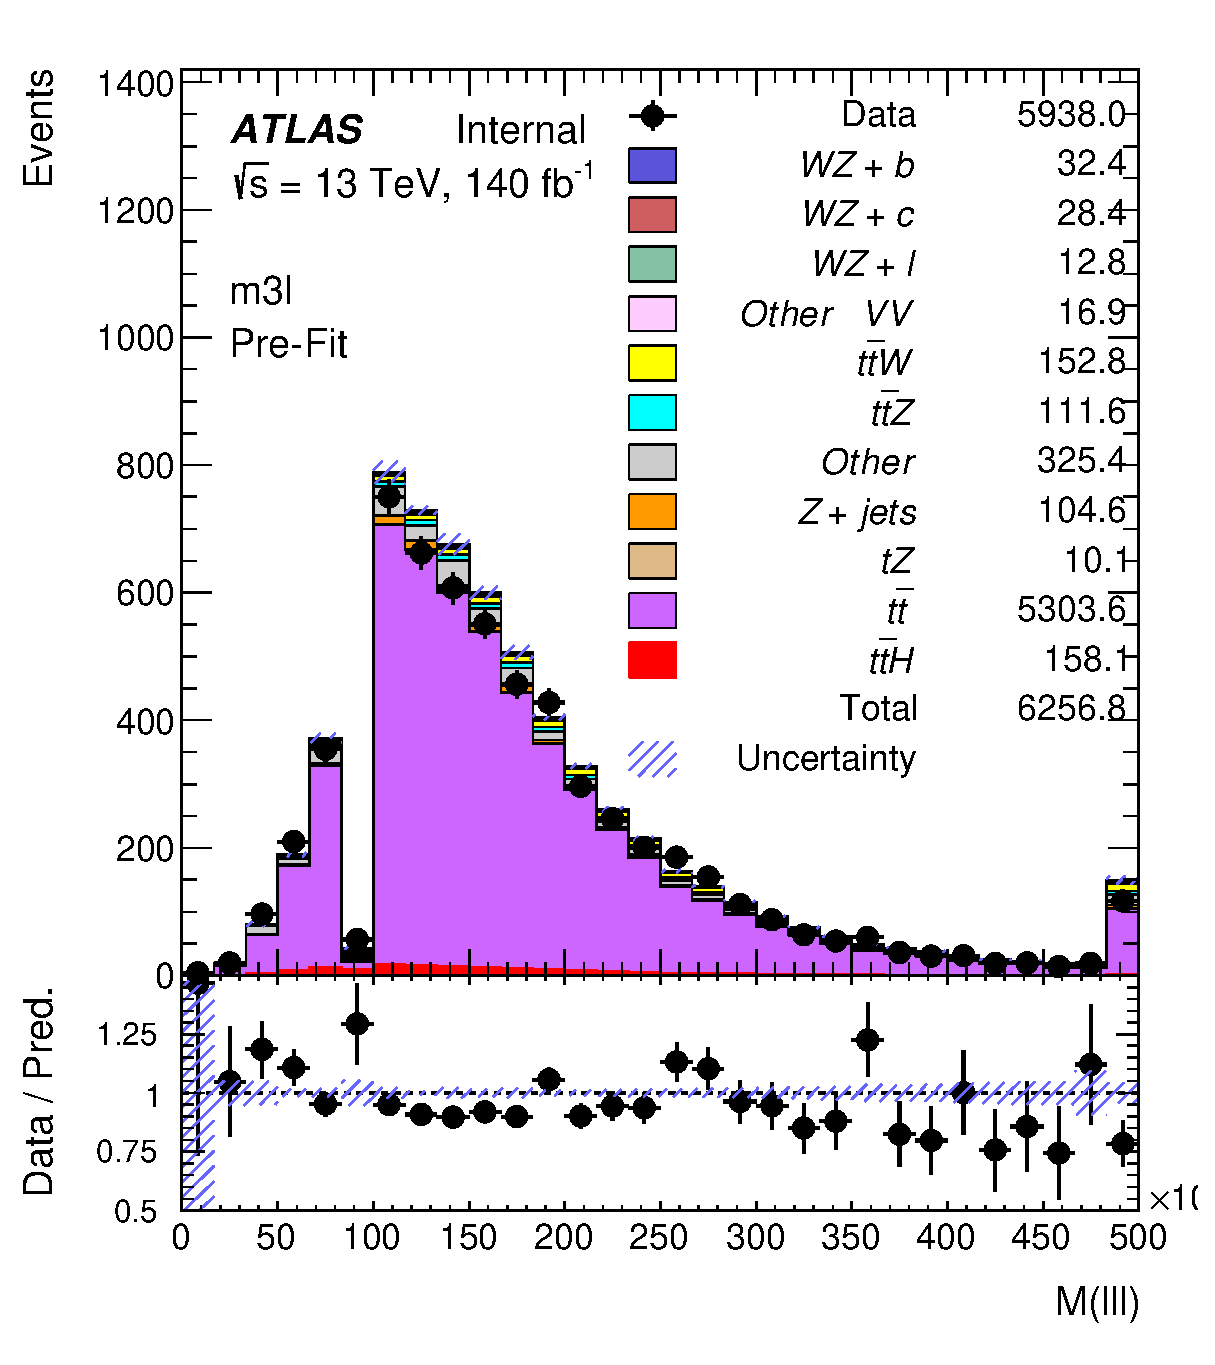
\includegraphics[width=0.48\textwidth]{kinematics/m3l.eps}}%
    \subfigure[]{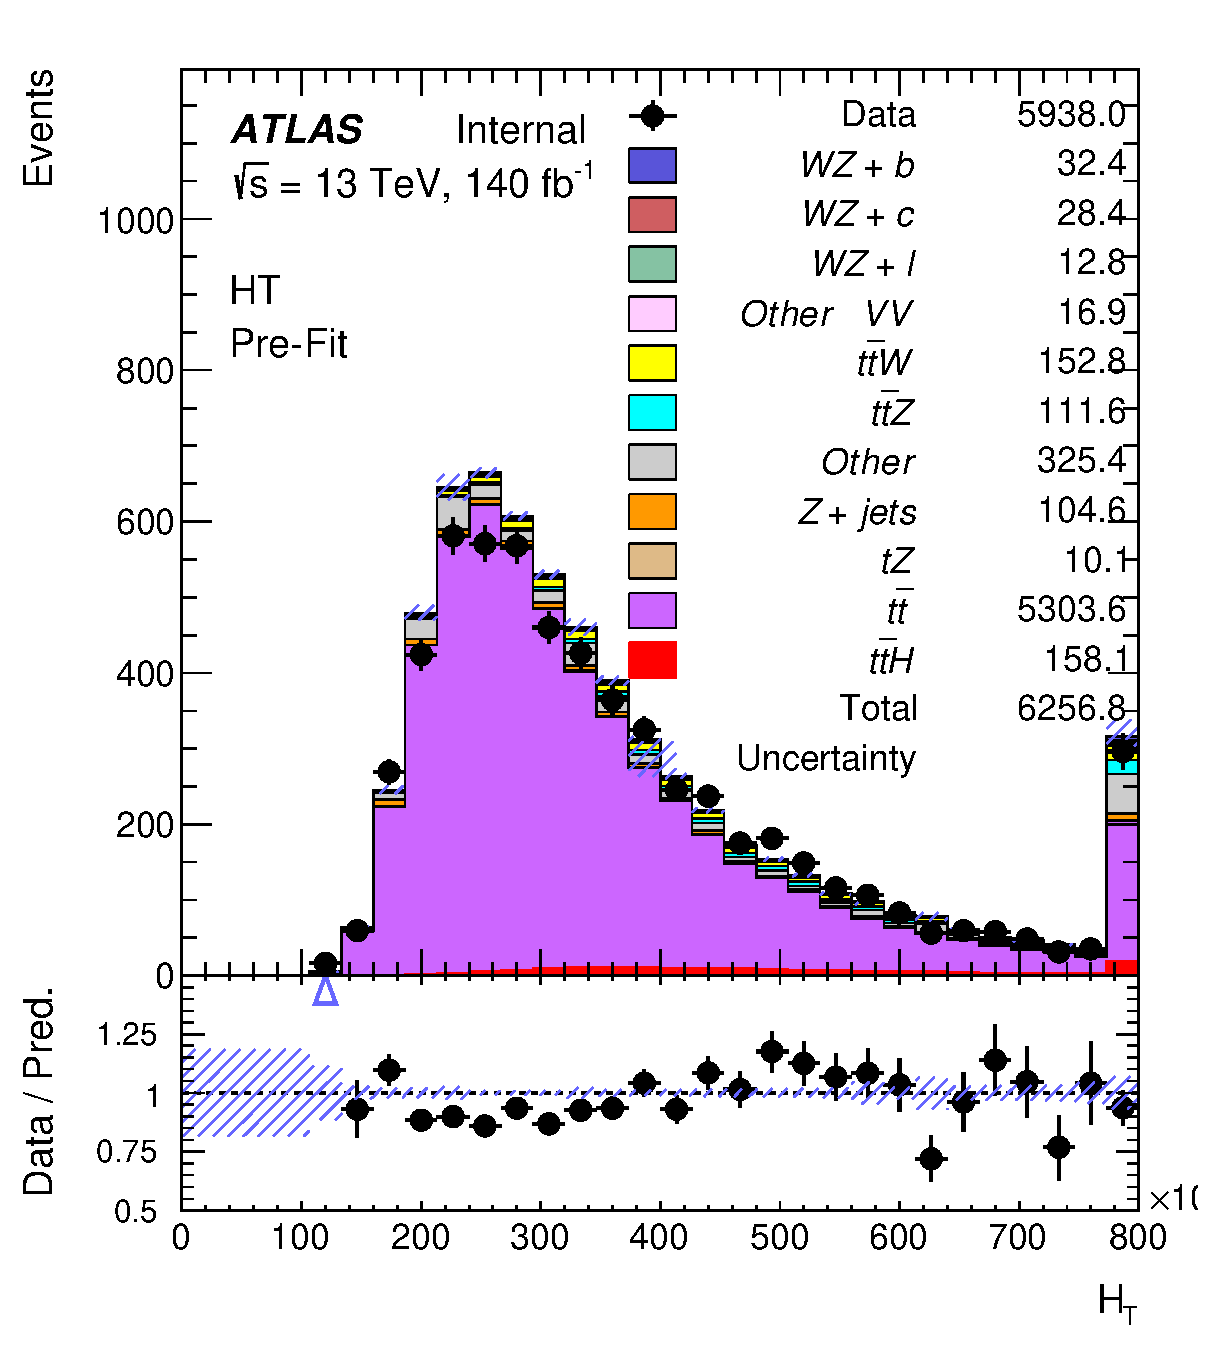
\includegraphics[width=0.48\textwidth]{kinematics/HT.eps}}\\
    \subfigure[]{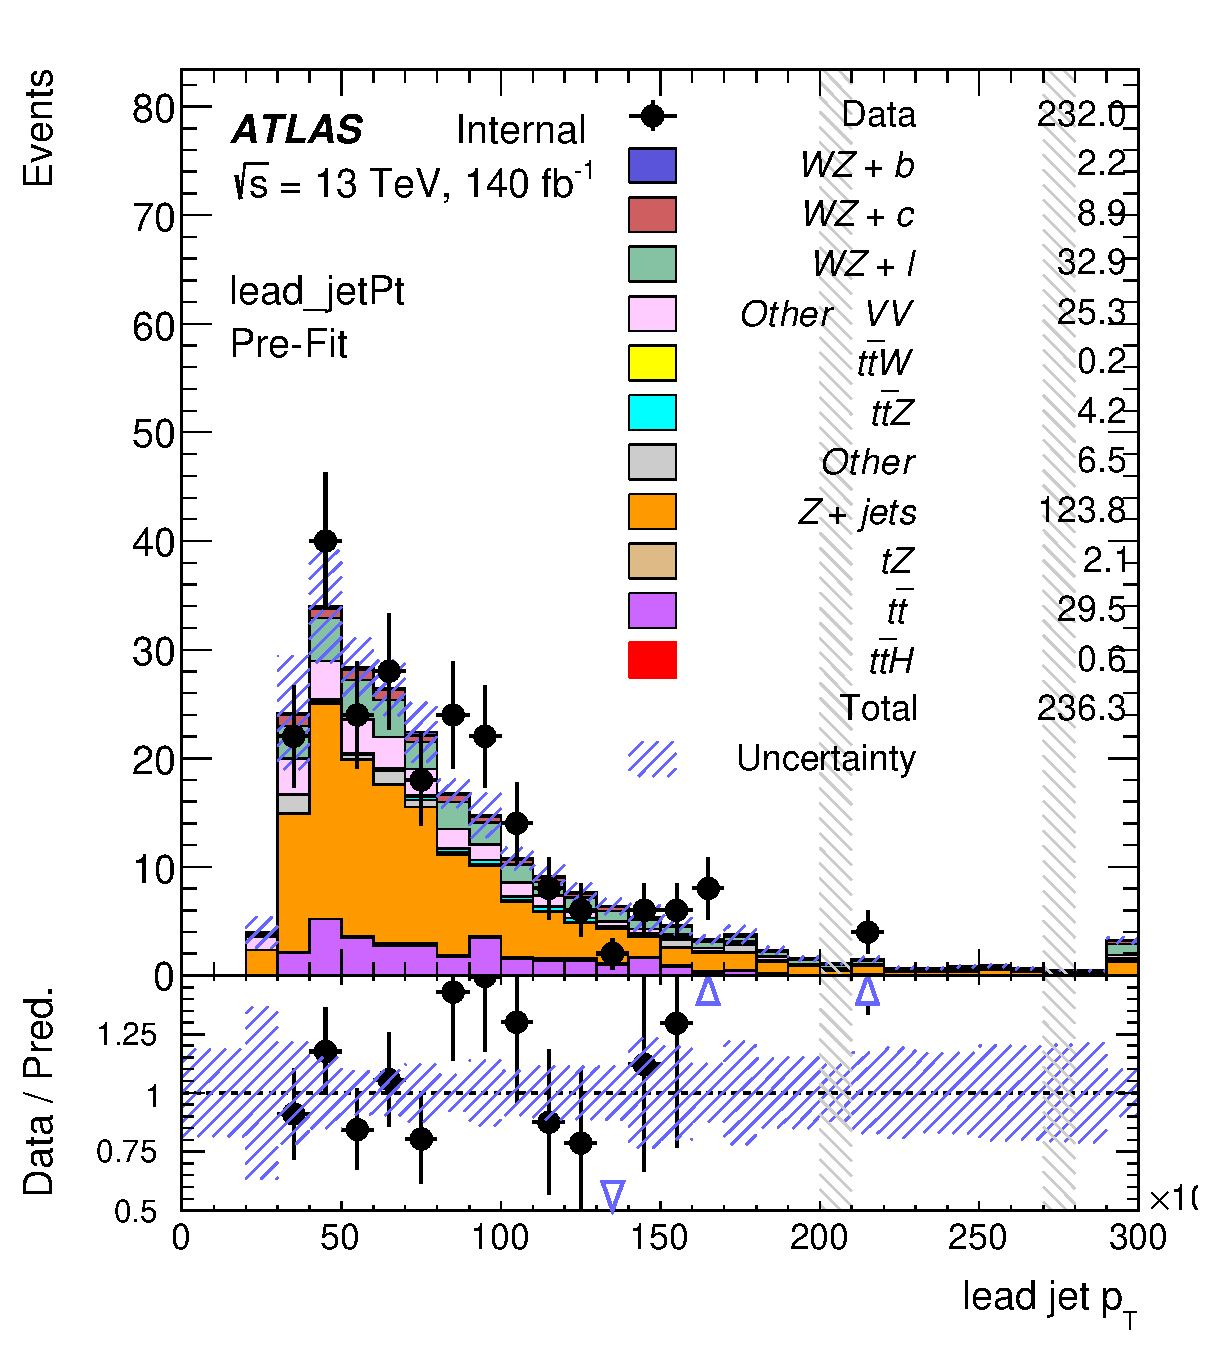
\includegraphics[width=0.48\textwidth]{kinematics/lead_jetPt.eps}}%
    \subfigure[]{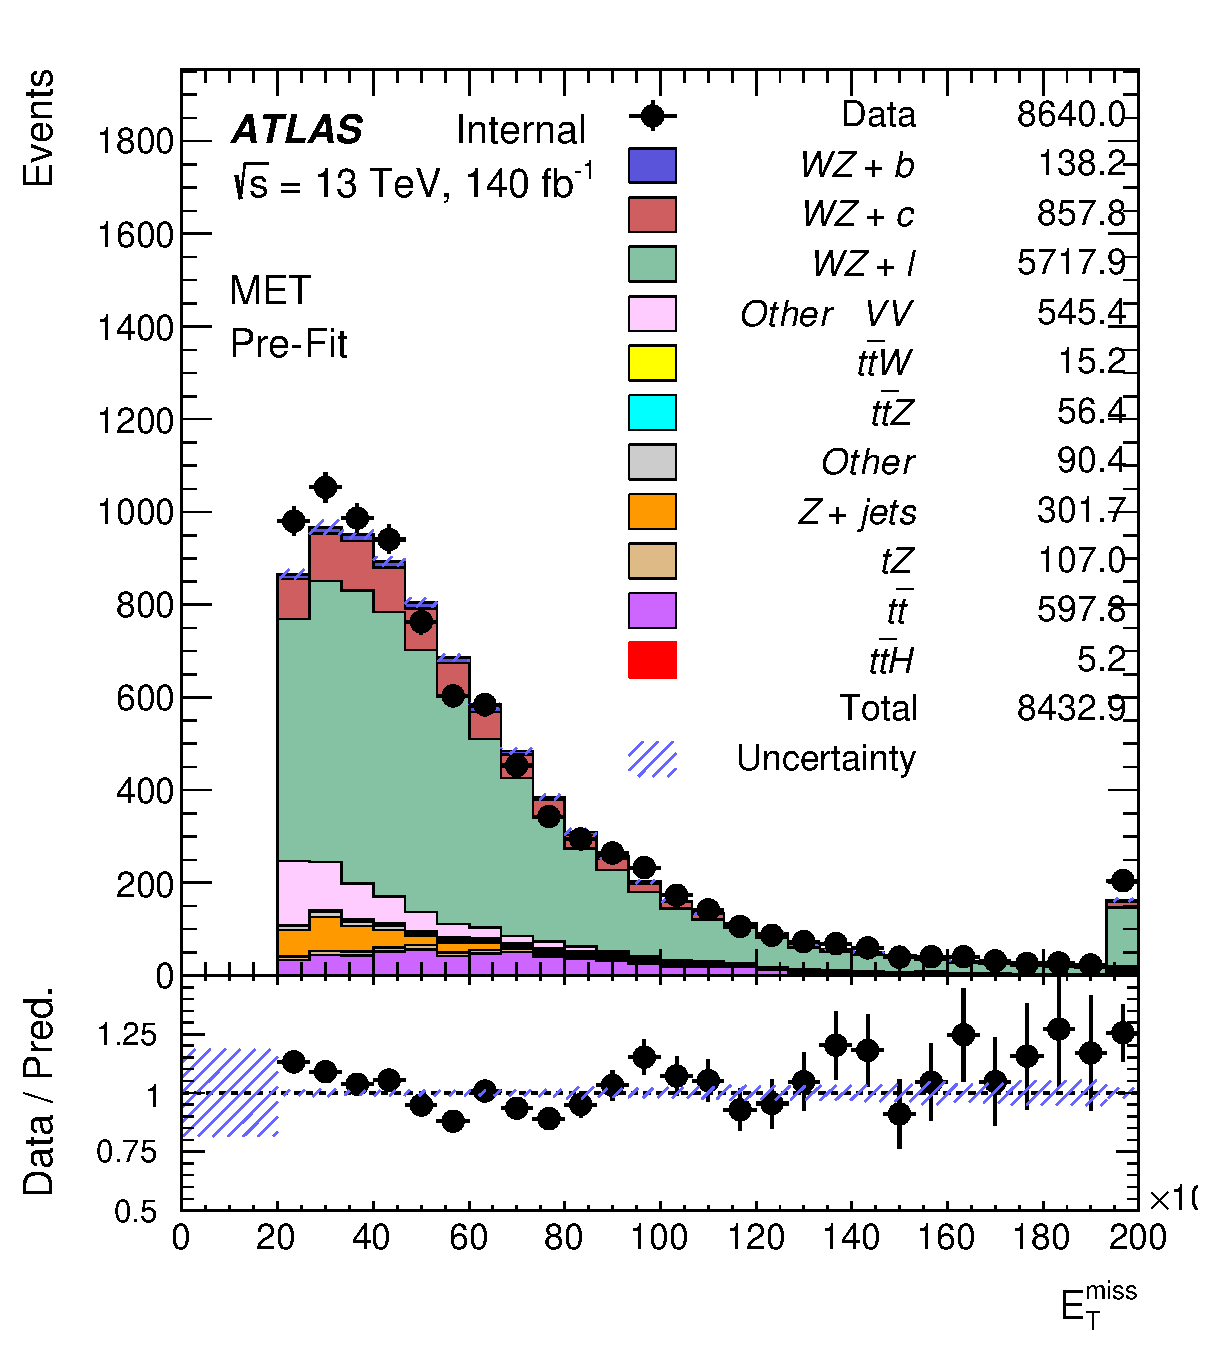
\includegraphics[width=0.48\textwidth]{kinematics/MET.eps}}\\
    \caption{Comparisons between the data and MC distributions in the signal region for (a) the invariant mass of the three leptons, (b) the $H_T$ of each event, (c) the $p_T$ of the leading jet, (d) the missing transverse energy.}    
\end{figure}
\begin{figure}[H]
    \subfigure[]{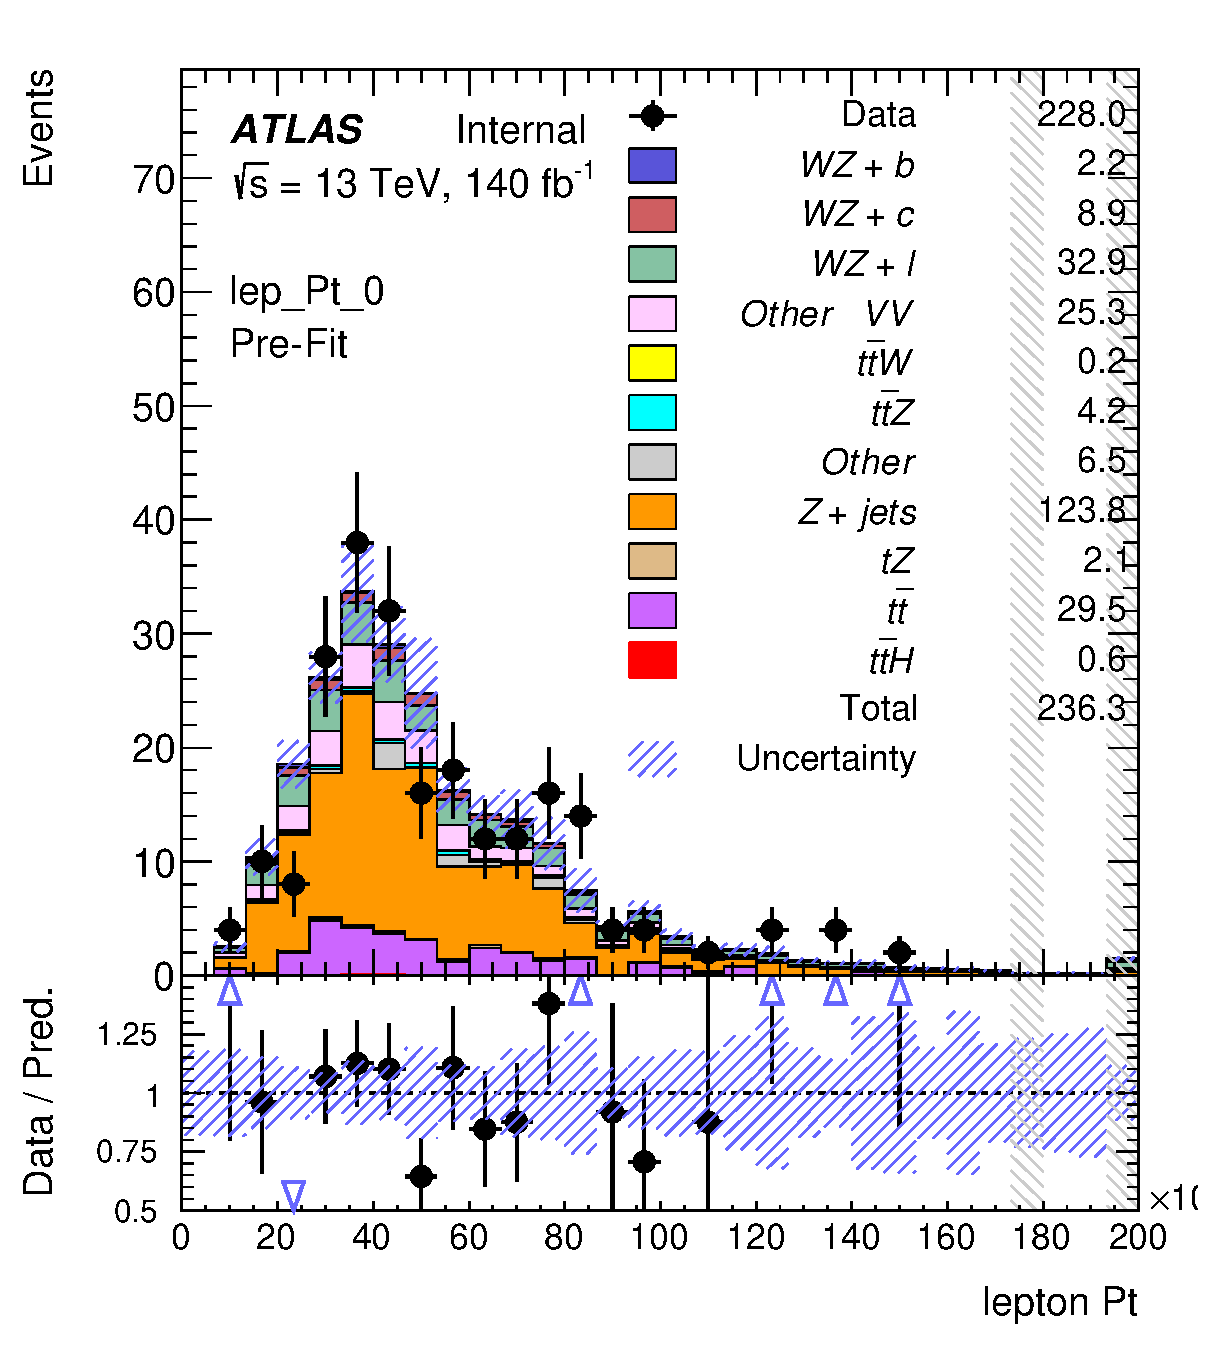
\includegraphics[width=0.48\textwidth]{kinematics/lep_Pt_0.eps}}%                                                             
    \subfigure[]{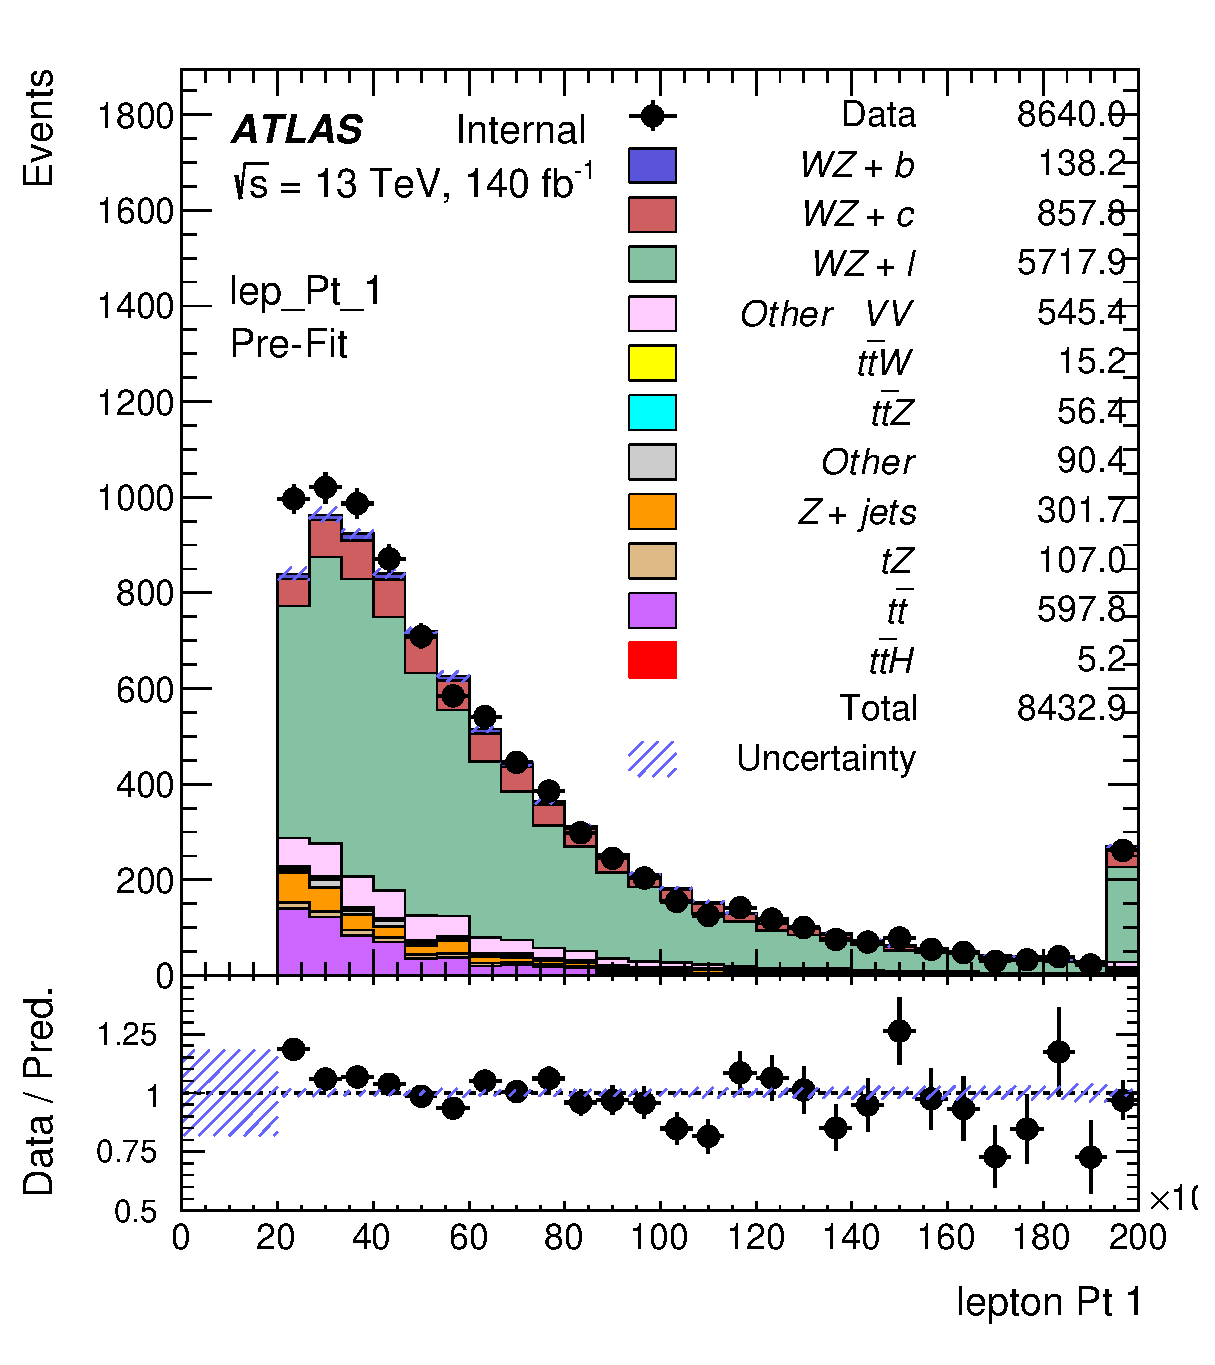
\includegraphics[width=0.48\textwidth]{kinematics/lep_Pt_1.eps}}\\
    \subfigure[]{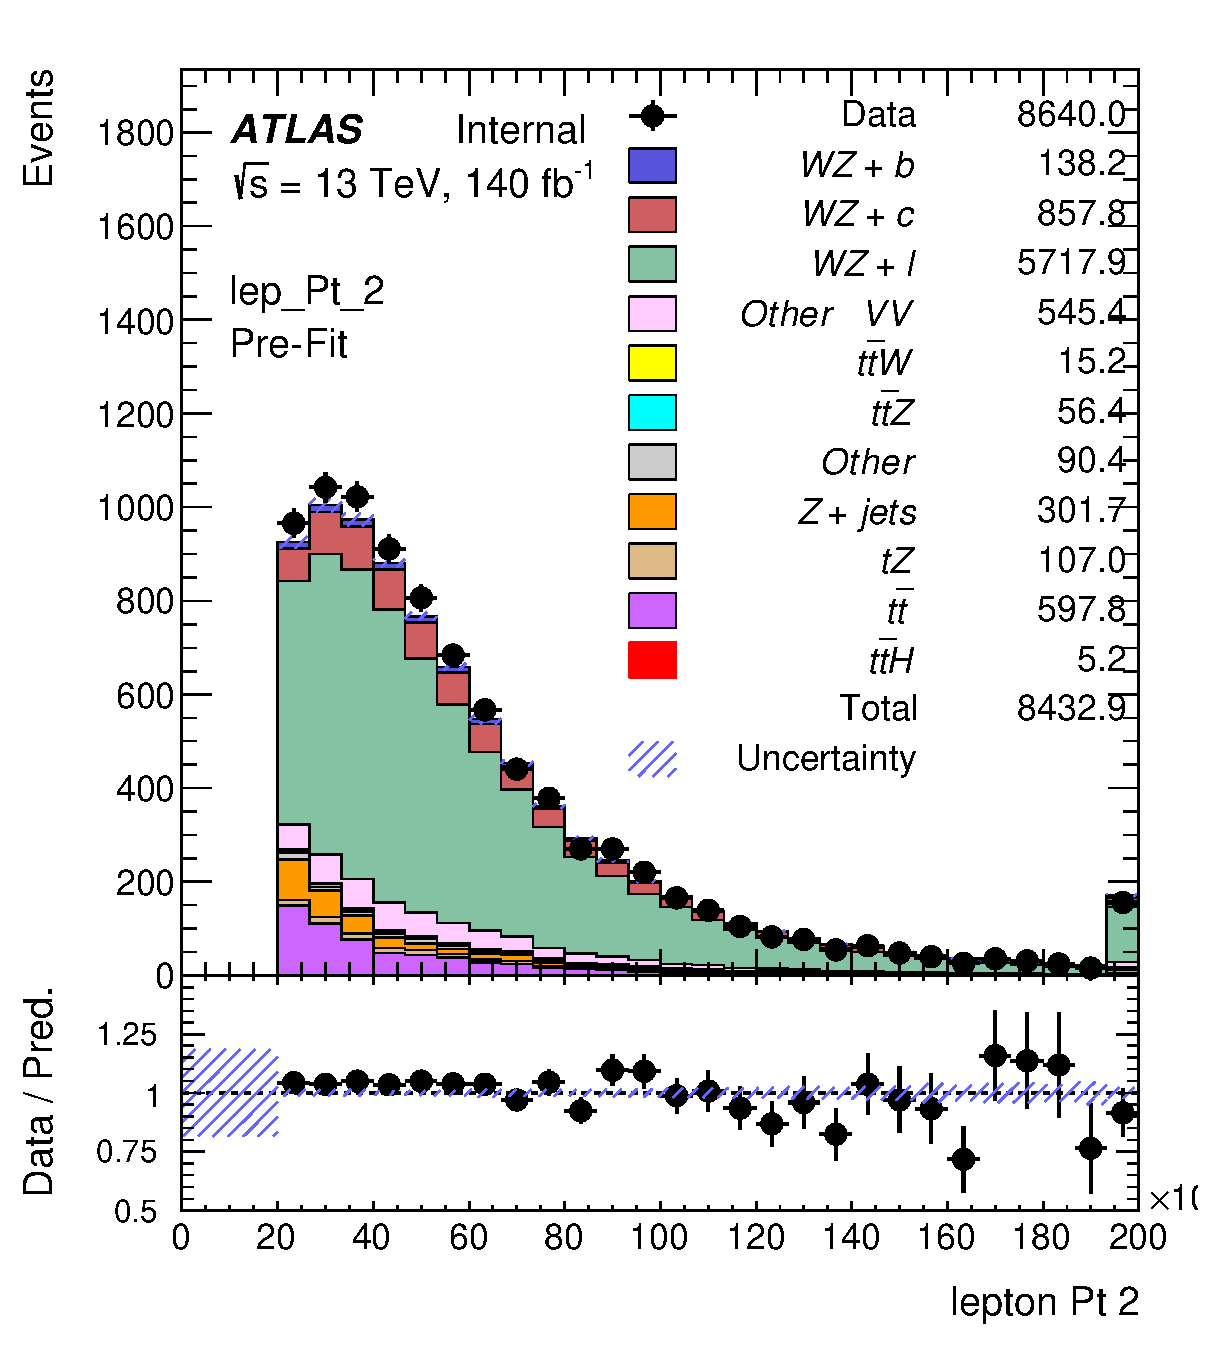
\includegraphics[width=0.48\textwidth]{kinematics/lep_Pt_2.eps}}%      
    \subfigure[]{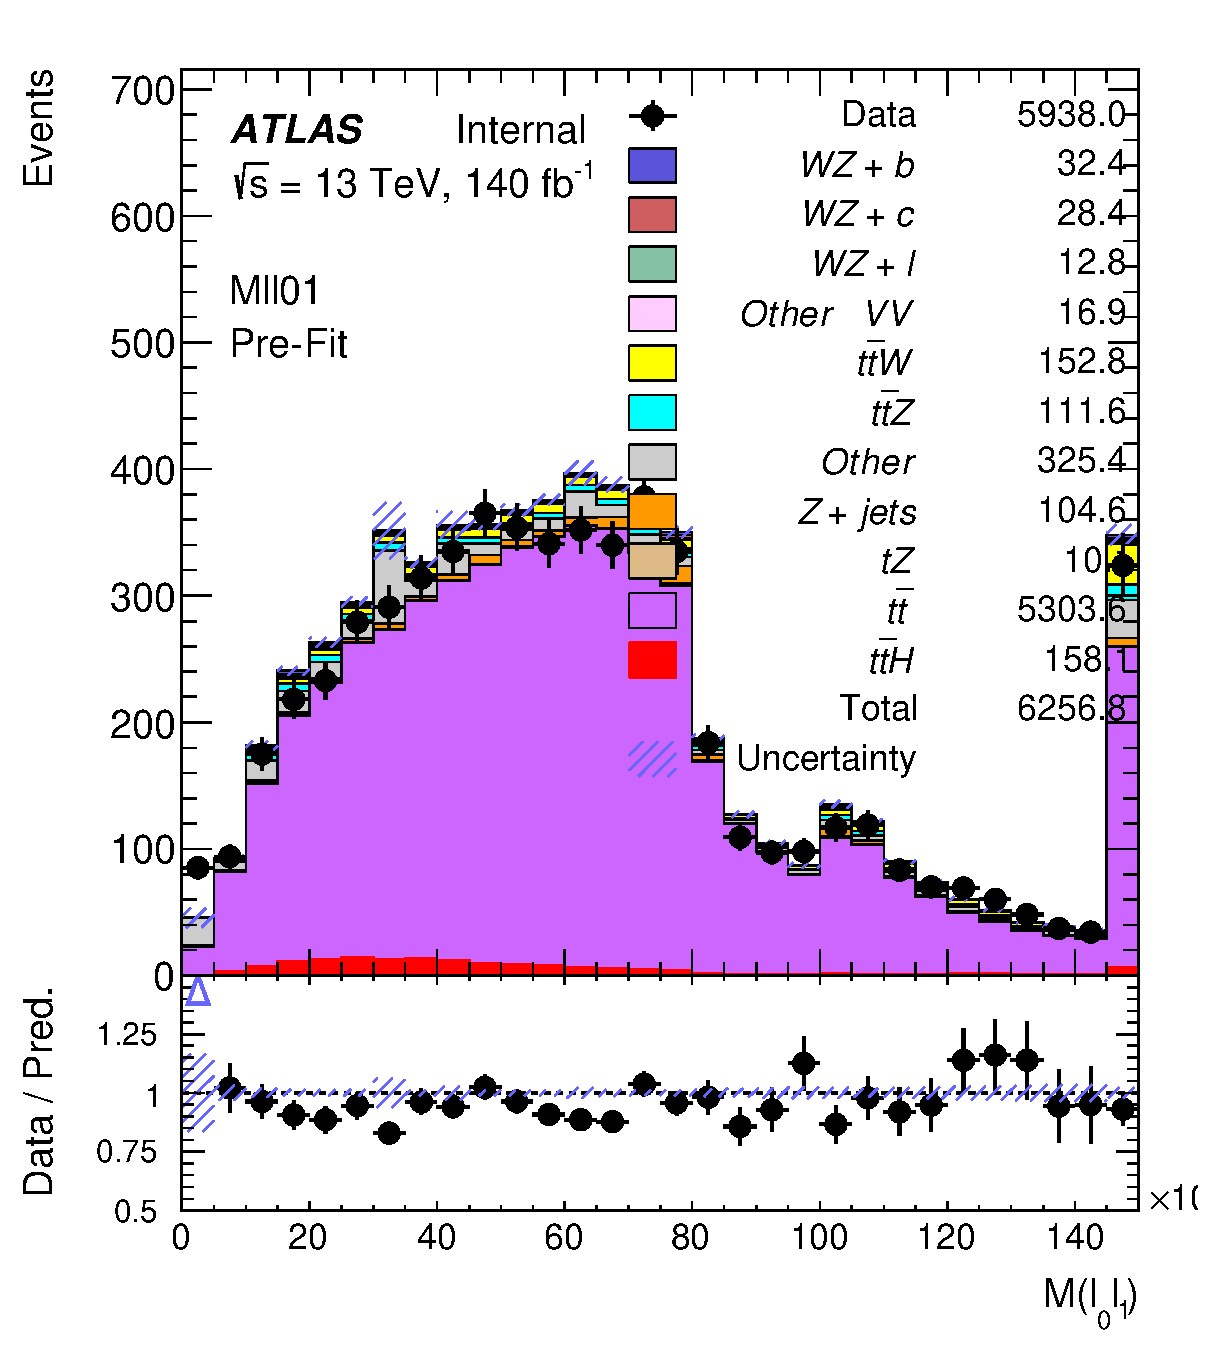
\includegraphics[width=0.48\textwidth]{kinematics/Mll01.eps}}\\
    \caption{Comparisons between the data and MC distributions in the signal region for (a) the transverse momentum of the opposite sign lepton, (b) the transverse momentum of the same-sign lepton closest to the opposite sign lepton, (c) the $p_T$ of the lepton furthest from the opposite sign lepton, (d) the invariant mass of lepton 0 and lepton 1.}
\end{figure}
\begin{figure}[H]
    \subfigure[]{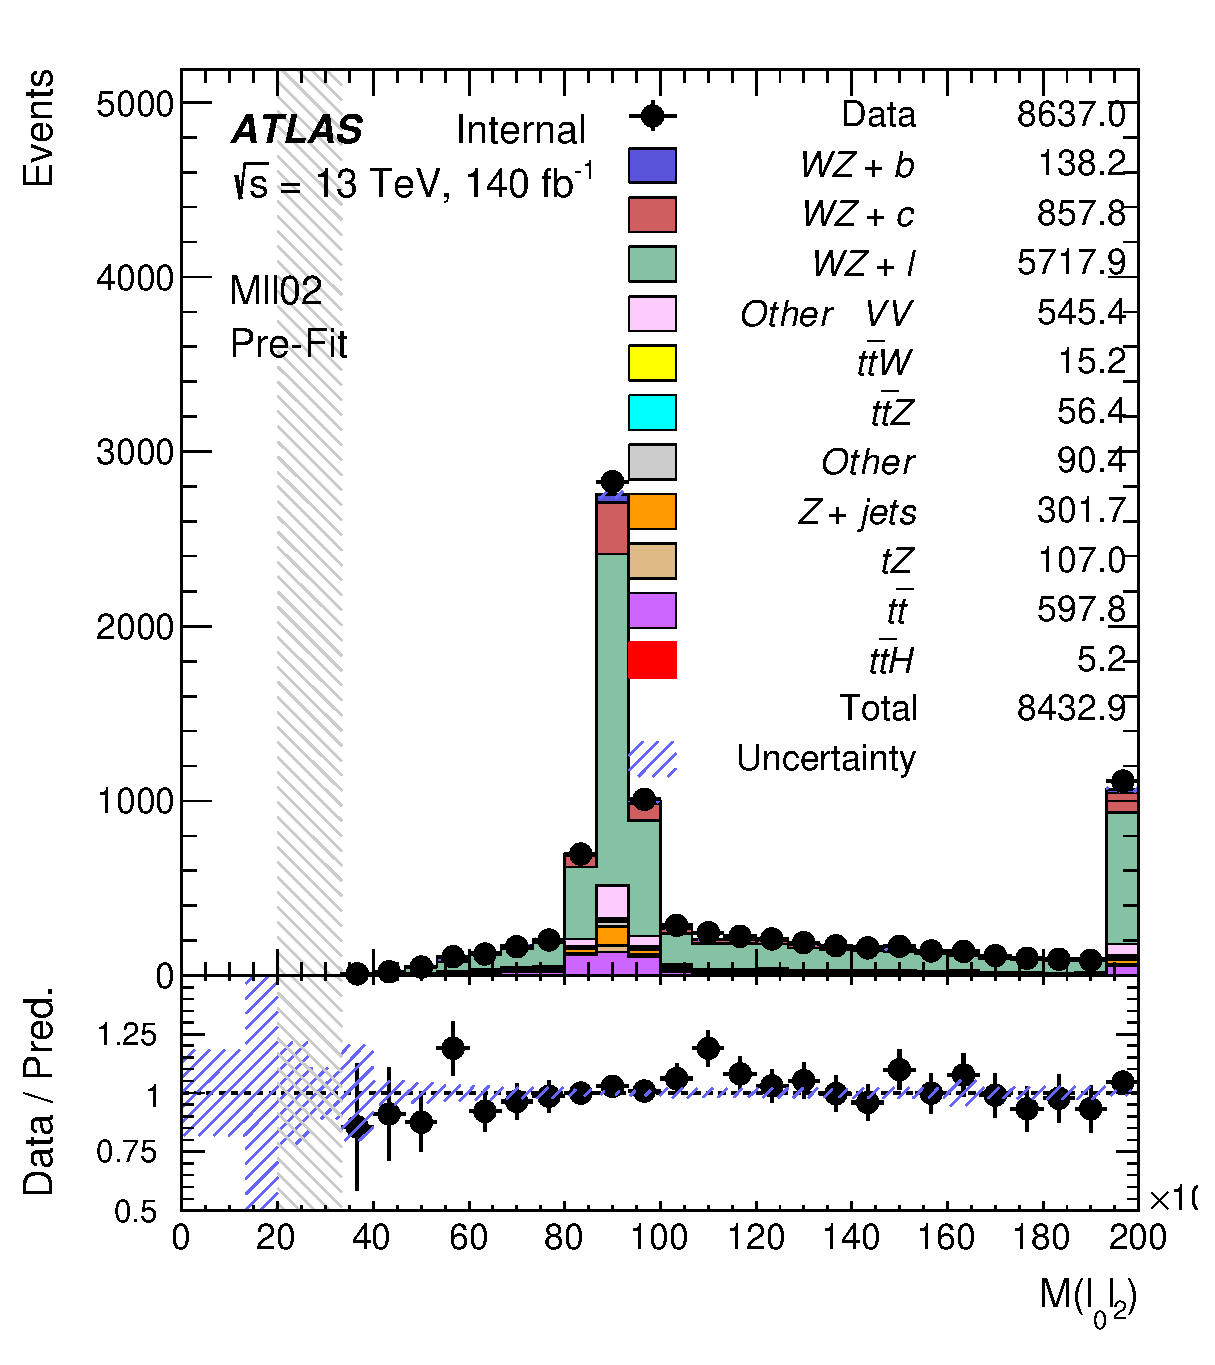
\includegraphics[width=0.48\textwidth]{kinematics/Mll02.eps}}%                                                      
    \subfigure[]{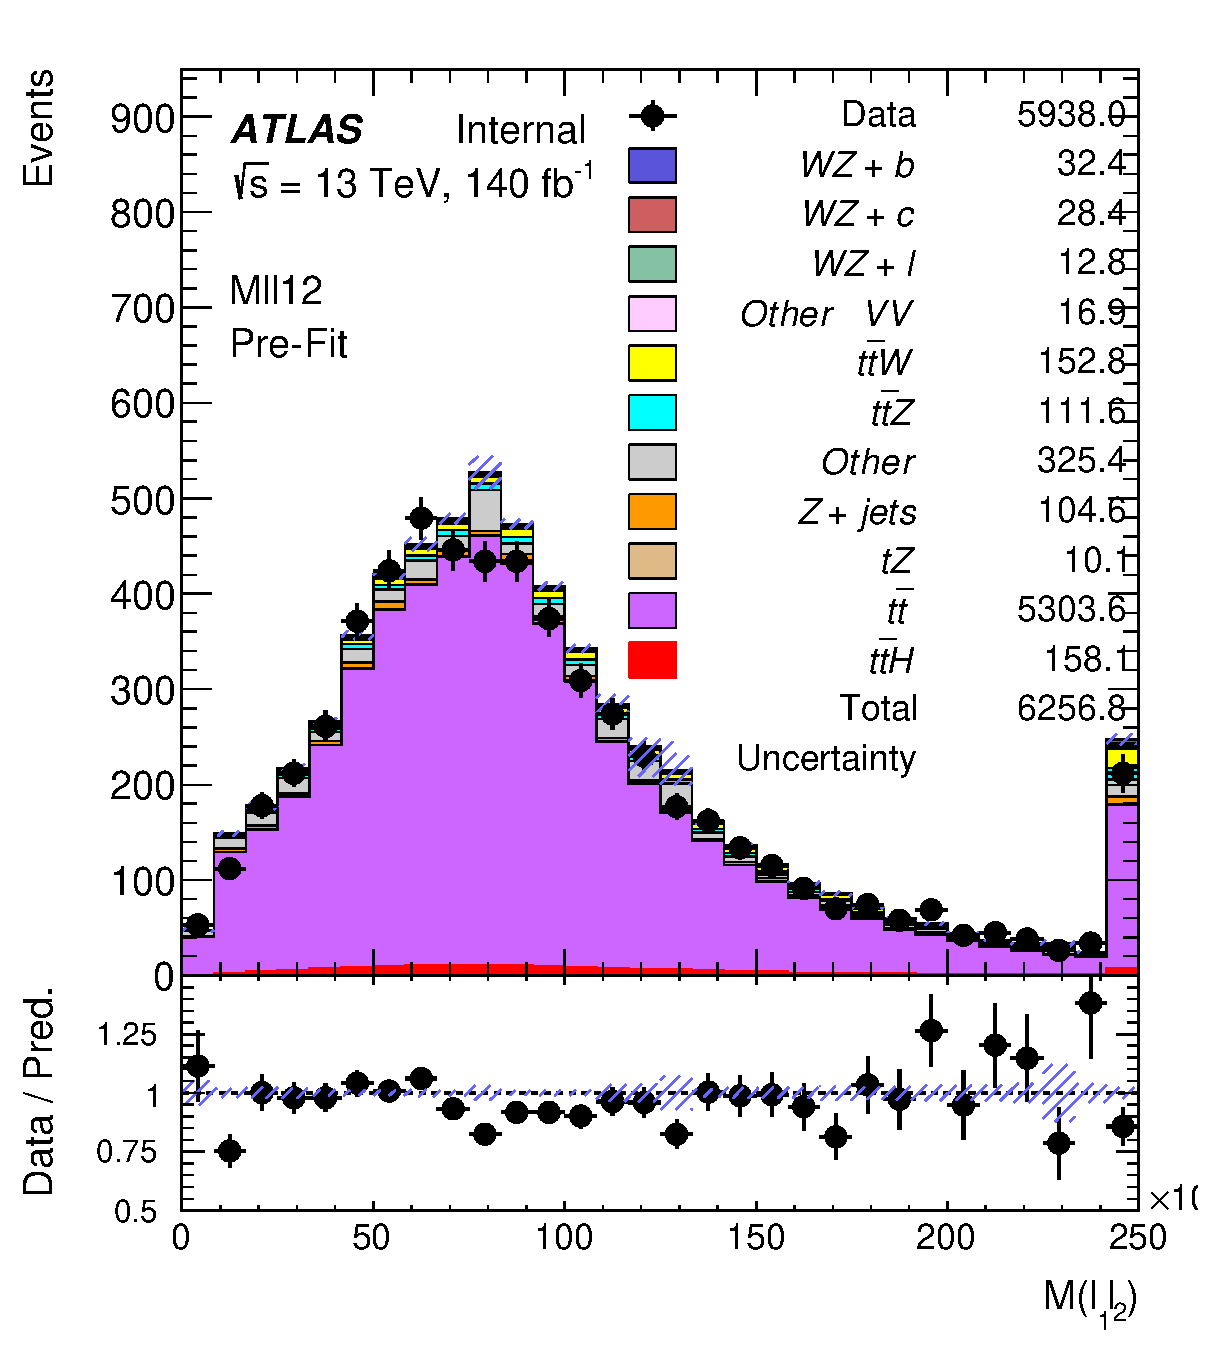
\includegraphics[width=0.48\textwidth]{kinematics/Mll12.eps}}\\
    \caption{Comparisons between the data and MC distributions in the signal region for (a) the invariant mass of leptons 0 and 2, (b) the invariant mass of the pair of leptons 1 and 2}
    \label{sr_kinematics}
\end{figure}

\begin{figure}%[h]
    \caption{WZ Fit Region - Inclusive}
    \subfigure[]{\includegraphics[width=.29\linewidth]{regions/plots_inclusive/Plots/lead_jetPt.png}}%
    \subfigure[]{\includegraphics[width=.29\linewidth]{regions/plots_inclusive/Plots/lep_Pt_0.png}}%
    \subfigure[]{\includegraphics[width=.29\linewidth]{regions/plots_inclusive/Plots/lep_Pt_1.png}}\\      
    \subfigure[]{\includegraphics[width=.29\linewidth]{regions/plots_inclusive/Plots/lep_Pt_2.png}}%
    \subfigure[]{\includegraphics[width=.29\linewidth]{regions/plots_inclusive/Plots/MET.png}}%
    \subfigure[]{\includegraphics[width=.29\linewidth]{regions/plots_inclusive/Plots/Mll01.png}}\\
    \label{kin:inclusive}
\end{figure}

\begin{figure}%[H]
    \caption{WZ Fit Region - 1j $<$ 85\% WP}
    \subfigure[]{\includegraphics[width=.29\linewidth]{regions/plots_not_85/Plots/lead_jetPt.png}}%
    \subfigure[]{\includegraphics[width=.29\linewidth]{regions/plots_not_85/Plots/lep_Pt_0.png}}%
    \subfigure[]{\includegraphics[width=.29\linewidth]{regions/plots_not_85/Plots/lep_Pt_1.png}}\\
    \subfigure[]{\includegraphics[width=.29\linewidth]{regions/plots_not_85/Plots/lep_Pt_2.png}}%
    \subfigure[]{\includegraphics[width=.29\linewidth]{regions/plots_not_85/Plots/MET.png}}%
    \subfigure[]{\includegraphics[width=.29\linewidth]{regions/plots_not_85/Plots/Mll01.png}}\\
    \label{kin:WP_1j_not85}
\end{figure}

\begin{figure}%[H]
    \caption{WZ Fit Region - 1j 77-85\% WP}
    \subfigure[]{\includegraphics[width=.29\linewidth]{regions/plots_1j_77_85/Plots/lead_jetPt.png}}%
    \subfigure[]{\includegraphics[width=.29\linewidth]{regions/plots_1j_77_85/Plots/lep_Pt_0.png}}%
    \subfigure[]{\includegraphics[width=.29\linewidth]{regions/plots_1j_77_85/Plots/lep_Pt_1.png}}\\
    \subfigure[]{\includegraphics[width=.29\linewidth]{regions/plots_1j_77_85/Plots/lep_Pt_2.png}}%
    \subfigure[]{\includegraphics[width=.29\linewidth]{regions/plots_1j_77_85/Plots/MET.png}}%
    \subfigure[]{\includegraphics[width=.29\linewidth]{regions/plots_1j_77_85/Plots/Mll01.png}}\\
    \label{kin:WP_1j_77_85}
\end{figure}

\begin{figure}%[H]
    \caption{WZ Fit Region - 1j 70-77\% WP}
    \subfigure[]{\includegraphics[width=.29\linewidth]{regions/plots_1j_70_77/Plots/lead_jetPt.png}}%
    \subfigure[]{\includegraphics[width=.29\linewidth]{regions/plots_1j_70_77/Plots/lep_Pt_0.png}}%
    \subfigure[]{\includegraphics[width=.29\linewidth]{regions/plots_1j_70_77/Plots/lep_Pt_1.png}}\\
    \subfigure[]{\includegraphics[width=.29\linewidth]{regions/plots_1j_70_77/Plots/lep_Pt_2.png}}%
    \subfigure[]{\includegraphics[width=.29\linewidth]{regions/plots_1j_70_77/Plots/MET.png}}%
    \subfigure[]{\includegraphics[width=.29\linewidth]{regions/plots_1j_70_77/Plots/Mll01.png}}\\
    \label{kin:WP_1j_70_77}   
\end{figure}

\begin{figure}%[H]
    \caption{WZ Fit Region - 1j 60-70\% WP}
    \subfigure[]{\includegraphics[width=.29\linewidth]{regions/plots_1j_60_70/Plots/lead_jetPt.png}}%
    \subfigure[]{\includegraphics[width=.29\linewidth]{regions/plots_1j_60_70/Plots/lep_Pt_0.png}}%
    \subfigure[]{\includegraphics[width=.29\linewidth]{regions/plots_1j_60_70/Plots/lep_Pt_1.png}}\\
    \subfigure[]{\includegraphics[width=.29\linewidth]{regions/plots_1j_60_70/Plots/lep_Pt_2.png}}%
    \subfigure[]{\includegraphics[width=.29\linewidth]{regions/plots_1j_60_70/Plots/MET.png}}%
    \subfigure[]{\includegraphics[width=.29\linewidth]{regions/plots_1j_60_70/Plots/Mll01.png}}\\
    \label{kin:WP_1j_60_70}
\end{figure}

\begin{figure}%[H]
    \caption{WZ Fit Region - 1j 60\% WP}
    \subfigure[]{\includegraphics[width=.29\linewidth]{regions/plots_1j_60/Plots/lead_jetPt.png}}%
    \subfigure[]{\includegraphics[width=.29\linewidth]{regions/plots_1j_60/Plots/lep_Pt_0.png}}%
    \subfigure[]{\includegraphics[width=.29\linewidth]{regions/plots_1j_60/Plots/lep_Pt_1.png}}\\
    \subfigure[]{\includegraphics[width=.29\linewidth]{regions/plots_1j_60/Plots/lep_Pt_2.png}}%
    \subfigure[]{\includegraphics[width=.29\linewidth]{regions/plots_1j_60/Plots/MET.png}}%
    \subfigure[]{\includegraphics[width=.29\linewidth]{regions/plots_1j_60/Plots/Mll01.png}}\\
    \label{kin:WP_1j_60}    
\end{figure}

\begin{figure}%[H]
    \caption{WZ Fit Region - tZ-CR}
    \subfigure[]{\includegraphics[width=.29\linewidth]{regions/plots_tZ_CR/Plots/lead_jetPt.png}}%
    \subfigure[]{\includegraphics[width=.29\linewidth]{regions/plots_tZ_CR/Plots/lep_Pt_0.png}}%
    \subfigure[]{\includegraphics[width=.29\linewidth]{regions/plots_tZ_CR/Plots/lep_Pt_1.png}}\\
    \subfigure[]{\includegraphics[width=.29\linewidth]{regions/plots_tZ_CR/Plots/lep_Pt_2.png}}%
    \subfigure[]{\includegraphics[width=.29\linewidth]{regions/plots_tZ_CR/Plots/MET.png}}%
    \subfigure[]{\includegraphics[width=.29\linewidth]{regions/plots_tZ_CR/Plots/Mll01.png}}\\
    \label{kin:tZ_CR_1j}
\end{figure}

\begin{figure}%[H]
    \caption{WZ Fit Region - 2j $<$ 85\% WP}
    \subfigure[]{\includegraphics[width=.29\linewidth]{regions/plots_not_85_2j/Plots/lead_jetPt.png}}%
    \subfigure[]{\includegraphics[width=.29\linewidth]{regions/plots_not_85_2j/Plots/lep_Pt_0.png}}%
    \subfigure[]{\includegraphics[width=.29\linewidth]{regions/plots_not_85_2j/Plots/lep_Pt_1.png}}\\
    \subfigure[]{\includegraphics[width=.29\linewidth]{regions/plots_not_85_2j/Plots/lep_Pt_2.png}}%
    \subfigure[]{\includegraphics[width=.29\linewidth]{regions/plots_not_85_2j/Plots/MET.png}}%
    \subfigure[]{\includegraphics[width=.29\linewidth]{regions/plots_not_85_2j/Plots/Mll01.png}}\\
    \label{kin:WP_2j_not85}
\end{figure}

\begin{figure}%[H]
    \caption{WZ Fit Region - 2j 77-85\% WP}
    \subfigure[]{\includegraphics[width=.29\linewidth]{regions/plots_2j_77_85/Plots/lead_jetPt.png}}%
    \subfigure[]{\includegraphics[width=.29\linewidth]{regions/plots_2j_77_85/Plots/lep_Pt_0.png}}%
    \subfigure[]{\includegraphics[width=.29\linewidth]{regions/plots_2j_77_85/Plots/lep_Pt_1.png}}\\
    \subfigure[]{\includegraphics[width=.29\linewidth]{regions/plots_2j_77_85/Plots/lep_Pt_2.png}}%
    \subfigure[]{\includegraphics[width=.29\linewidth]{regions/plots_2j_77_85/Plots/MET.png}}%
    \subfigure[]{\includegraphics[width=.29\linewidth]{regions/plots_2j_77_85/Plots/Mll01.png}}\\
    \label{kin:WP_2j_77_85}
\end{figure}

\begin{figure}%[H]
    \caption{WZ Fit Region - 2j 70-77\% WP}
    \subfigure[]{\includegraphics[width=.29\linewidth]{regions/plots_2j_70_77/Plots/lead_jetPt.png}}%
    \subfigure[]{\includegraphics[width=.29\linewidth]{regions/plots_2j_70_77/Plots/lep_Pt_0.png}}%
    \subfigure[]{\includegraphics[width=.29\linewidth]{regions/plots_2j_70_77/Plots/lep_Pt_1.png}}\\
    \subfigure[]{\includegraphics[width=.29\linewidth]{regions/plots_2j_70_77/Plots/lep_Pt_2.png}}%
    \subfigure[]{\includegraphics[width=.29\linewidth]{regions/plots_2j_70_77/Plots/MET.png}}%
    \subfigure[]{\includegraphics[width=.29\linewidth]{regions/plots_2j_70_77/Plots/Mll01.png}}\\
    \label{kin:WP_2j_70_77}
\end{figure}

\begin{figure}%[H]
    \caption{WZ Fit Region - 2j 60-70\% WP}
    \subfigure[]{\includegraphics[width=.29\linewidth]{regions/plots_2j_60_70/Plots/lead_jetPt.png}}%
    \subfigure[]{\includegraphics[width=.29\linewidth]{regions/plots_2j_60_70/Plots/lep_Pt_0.png}}%
    \subfigure[]{\includegraphics[width=.29\linewidth]{regions/plots_2j_60_70/Plots/lep_Pt_1.png}}\\
    \subfigure[]{\includegraphics[width=.29\linewidth]{regions/plots_2j_60_70/Plots/lep_Pt_2.png}}%
    \subfigure[]{\includegraphics[width=.29\linewidth]{regions/plots_2j_60_70/Plots/MET.png}}%
    \subfigure[]{\includegraphics[width=.29\linewidth]{regions/plots_2j_60_70/Plots/Mll01.png}}\\
    \label{kin:WP_2j_60_70}
\end{figure}

\begin{figure}%[H]
    \caption{WZ Fit Region - 2j 60\% WP}
    \subfigure[]{\includegraphics[width=.29\linewidth]{regions/plots_2j_60/Plots/lead_jetPt.png}}%
    \subfigure[]{\includegraphics[width=.29\linewidth]{regions/plots_2j_60/Plots/lep_Pt_0.png}}%
    \subfigure[]{\includegraphics[width=.29\linewidth]{regions/plots_2j_60/Plots/lep_Pt_1.png}}\\
    \subfigure[]{\includegraphics[width=.29\linewidth]{regions/plots_2j_60/Plots/lep_Pt_2.png}}%
    \subfigure[]{\includegraphics[width=.29\linewidth]{regions/plots_2j_60/Plots/MET.png}}%
    \subfigure[]{\includegraphics[width=.29\linewidth]{regions/plots_2j_60/Plots/Mll01.png}}\\
    \label{kin:WP_2j_60}
\end{figure}

%\begin{figure}[H]
%    \caption{WZ Fit Region - tZ-CR-2j}
%    \subfigure[]{\includegraphics[width=.29\linewidth]{regions/plots_tZ_CR_2j/Plots/lead_jetPt.png}}%
%    \subfigure[]{\includegraphics[width=.29\linewidth]{regions/plots_tZ_CR_2j/Plots/lep_Pt_0.png}}%
%    \subfigure[]{\includegraphics[width=.29\linewidth]{regions/plots_tZ_CR_2j/Plots/lep_Pt_1.png}}\\
%    \subfigure[]{\includegraphics[width=.29\linewidth]{regions/plots_tZ_CR_2j/Plots/lep_Pt_2.png}}%
%    \subfigure[]{\includegraphics[width=.29\linewidth]{regions/plots_tZ_CR_2j/Plots/MET.png}}%
%    \subfigure[]{\includegraphics[width=.29\linewidth]{regions/plots_tZ_CR_2j/Plots/Mll01.png}}\\
%    \label{kin:tZ_CR_2j}
%\end{figure}

%---------------------------
\subsection{Non-Prompt Lepton Estimation}
\label{sec:fakes}
%---------------------------

Two processes act as sources of non-prompt leptons appear in the analysis: $t\bar{t}$ and $Z$+jet production both produce two prompt leptons, and each contribute to the signal region when an additional non-prompt lepton appears in the event. The contribution of these processes is estimated with Monte Carlo simulations, which are validated using enriched validation regions.

\subsubsection{$t\bar{t}$ Validation}

$t\bar{t}$ events can produce two prompt leptons from the decay of each of the tops. These top decays produce two b-quarks, the decay of which can produce additional non-prompt leptons, which occasionally pass the selection of the signal region. In order to validate that the Monte Carlo accurately simulates this process accurately, the MC prediction in a non-prompt $t\bar{t}$ enriched validation region is compared to data.

The $t\bar{t}$ validation region is similar to the signal region - three leptons meeting the criteria described in section \ref{sec:evt_selection} are required, and the requirements on $E_T^{miss}$ remain the same. However, the selection requiring a lepton pair form a Z-candidate are reversed. Events where the invariant mass of any two opposite sign, same flavor leptons falls within 10 GeV of 91.2 GeV are rejected. This ensures the $t\bar{t}$ validation region is orthogonal to the signal region. 

Further, because the jet multiplicity of $t\bar{t}$ events tends to be higher than WZ, the number of jets in each event is required to be greater than 1. As b-jets are almost invariably produced from top decays, at least one b-tagged jet in each event is required. 

%This selection creates a region which is dominated by $t\bar{t}$ events. The yields in this region are summarized in \ref{tab:ttbar_yields}.

%\begin{table}[H]
%    \centering
%        %\input{ttbar_yields.tex}
%    \caption{Data and MC yields after the event selection of the $t\bar{t}$ validation region has been applied.}
%    \label{tab:ttbar_yields}
%\end{table}

Various kinematic plots of this region are shown below. The general agreement between data and MC in each of these suggests that the non-prompt contribution of $t\bar{t}$ is well modeled by Monte Carlo.

\begin{figure}[H]
    \subfigure[]{\includegraphics[width=0.48\textwidth]{ttbar/m3l.png}}%                                                 
    \subfigure[]{\includegraphics[width=0.48\textwidth]{ttbar/HT.png}}\\
    \subfigure[]{\includegraphics[width=0.48\textwidth]{ttbar/lead_jetPt.png}}%                             
    \subfigure[]{\includegraphics[width=0.48\textwidth]{ttbar/MET.png}}\\
    \caption{Comparisons between the data and MC distributions in the $t\bar{t}$ validation region for (a) the invariant mass of the three leptons, (b) the $H_T$ of each event, (c) the $p_T$ of the leading jet, (d) the missing transverse energy.}    
    \end{figure}
\begin{figure}[H]
    \subfigure[]{\includegraphics[width=0.48\textwidth]{ttbar/lep_Pt_0.png}}%                                                              
    \subfigure[]{\includegraphics[width=0.48\textwidth]{ttbar/lep_Pt_1.png}}\\
    \subfigure[]{\includegraphics[width=0.48\textwidth]{ttbar/lep_Pt_2.png}}%                                                              
    \subfigure[]{\includegraphics[width=0.48\textwidth]{ttbar/Mll01.png}}\\
    \caption{Comparisons between the data and MC distributions in the $t\bar{t}$ validation region for (a) the transverse momentum of the opposite sign lepton, (b) the transverse momentum of the same-sign lepton closest to the opposite sign lepton, (c) the $p_T$ of the lepton furthest from the opposite sign lepton, (d) the invariant mass of lepton 0 and lepton 1.}
\end{figure}
\begin{figure}[H]
    \subfigure[]{\includegraphics[width=0.48\textwidth]{ttbar/nJets_OR.png}}%                                                               
    \subfigure[]{\includegraphics[width=0.48\textwidth]{ttbar/nJets_OR_DL1r_70.png}}\\
    \caption{Comparisons between the data and MC distributions in the $t\bar{t}$ validation region for (a) the number of jets, (b) the number of b-tagged jets.}
    \label{ttbar_kinematics}
\end{figure}

\subsubsection{$Z$+jets Validation}

Similar to $t\bar{t}$, a non-prompt $Z$+jets validation region is produced in order to validate the MC predictions. The lepton requirements remain the same as the signal region. Because no neutrinos are present for this process, the $E_T^{miss}$ cut is reversed, requiring $E_T^{miss}$ < 30 GeV. This also ensures this validation region is orthogonal to the signal region. Further, the number of jets in each event is required to be greater than one. 

Various kinematic plots of this region are shown below. The general agreement between data and MC in each of these suggests that the non-prompt contribution of $Z$+jets is well modeled by Monte Carlo.

\begin{figure}[H]
    \subfigure[]{\includegraphics[width=0.48\textwidth]{zjets/m3l.png}}%                                                    
    \subfigure[]{\includegraphics[width=0.48\textwidth]{zjets/HT.png}}\\
    \subfigure[]{\includegraphics[width=0.48\textwidth]{zjets/lead_jetPt.png}}%                                                        
    \subfigure[]{\includegraphics[width=0.48\textwidth]{zjets/MET.png}}\\
    \caption{Comparisons between the data and MC distributions in the $t\bar{t}$ validation region for (a) the invariant mass of the three leptons, (b) the $H_T$ of each event, (c) the $p_T$ of the leading jet, (d) the missing transverse energy.}    
    \end{figure}
\begin{figure}[H]
    \subfigure[]{\includegraphics[width=0.48\textwidth]{zjets/lep_Pt_0.png}}%                                                                   
    \subfigure[]{\includegraphics[width=0.48\textwidth]{zjets/lep_Pt_1.png}}\\
    \subfigure[]{\includegraphics[width=0.48\textwidth]{zjets/lep_Pt_2.png}}%                                                                   
    \subfigure[]{\includegraphics[width=0.48\textwidth]{zjets/Mll01.png}}\\
    \caption{Comparisons between the data and MC distributions in the $Z$+jets validation region for (a) the transverse momentum of the opposite sign lepton, (b) the transverse momentum of the same-sign lepton closest to the opposite sign lepton, (c) the $p_T$ of the lepton furthest from the opposite sign lepton, (d) the invariant mass of lepton 0 and lepton 1.}
\end{figure}
\begin{figure}[H]
    \subfigure[]{\includegraphics[width=0.48\textwidth]{zjets/nJets_OR.png}}%                                                                
    \subfigure[]{\includegraphics[width=0.48\textwidth]{zjets/nJets_OR_DL1r_70.png}}\\
    \caption{Comparisons between the data and MC distributions in the $Z$+jets validation region for (a) the number of jets, (b) the number of b-tagged jets.}
    \label{zjets_kinematics}
\end{figure}

